\subsection{Fase 1 (2018-12-04 - 2019-01-21)}
	\subsubsection{Ore impiegate}
	La seguente tabella indica le ore impiegate durante la fase 1. Tra parentesi viene indicata la differenza tra ore preventivate e ore impiegate ($preventivo - consuntivo$): valori positivi indicano le ore risparmiate e valori negativi indicano le ore in eccesso.
	
	\begin{table}[H]
		\centering
		\begin{tabular}{| l | c c c c c c | c |}
			\rowcolor{LightBlue}
			& \multicolumn{7}{c}{\textbf{\color{white}Numero di ore}}	\\	
			\rowcolor{LightBlue}
			\textbf{\color{white}Membro}
			& \textbf{\color{white}RES}
			& \textbf{\color{white}AMM}
			& \textbf{\color{white}AN}
			& \textbf{\color{white}PRO}
			& \textbf{\color{white}DEV}
			& \textbf{\color{white}VER}
			& \textbf{\color{white}Totali}\\	
			Bergo     		& -  (0)		& 9  (+6) 	& 22 (-8) 		& - (0) & - (0) & 7  (+1) 	& 38\\
			Bortone   		& -  (0)		& 14 (-4) 	& 18 (-3) 		& - (0) & - (0) & 10 (-2)	& 42\\
			Cosentino 		& 25 (-5) 	& -  (0) 	& 24 (-2) 		& - (0) & - (0) & -  (+5)	& 49\\
			Marcato   		& 10 (-5) 	& 10 (0) 	& 22 (+3) 		& - (0) & - (0) & -  (+3)	& 42\\
			Peagno    		& -  (+5) 	& 15 (0) 	& 23 (-1) 		& - (0) & - (0) & -  (+3)	& 38\\
			Peron     		& -  (0)		& 13 (-3) 	& 23 (+6) 		& - (0) & - (0) & 13 (-8)	& 49\\
			Pettenuzzo 	& - (0) 		& 12 (+3) 	& 5  (+14) 	& - (0) & - (0) & 13 (-8)	& 30\\ \hline
		\end{tabular}
		\caption{Ore di lavoro impiegate per membro/ruolo della fase 1}
	\end{table}
	
	\begin{figure}[H]
		\centering
		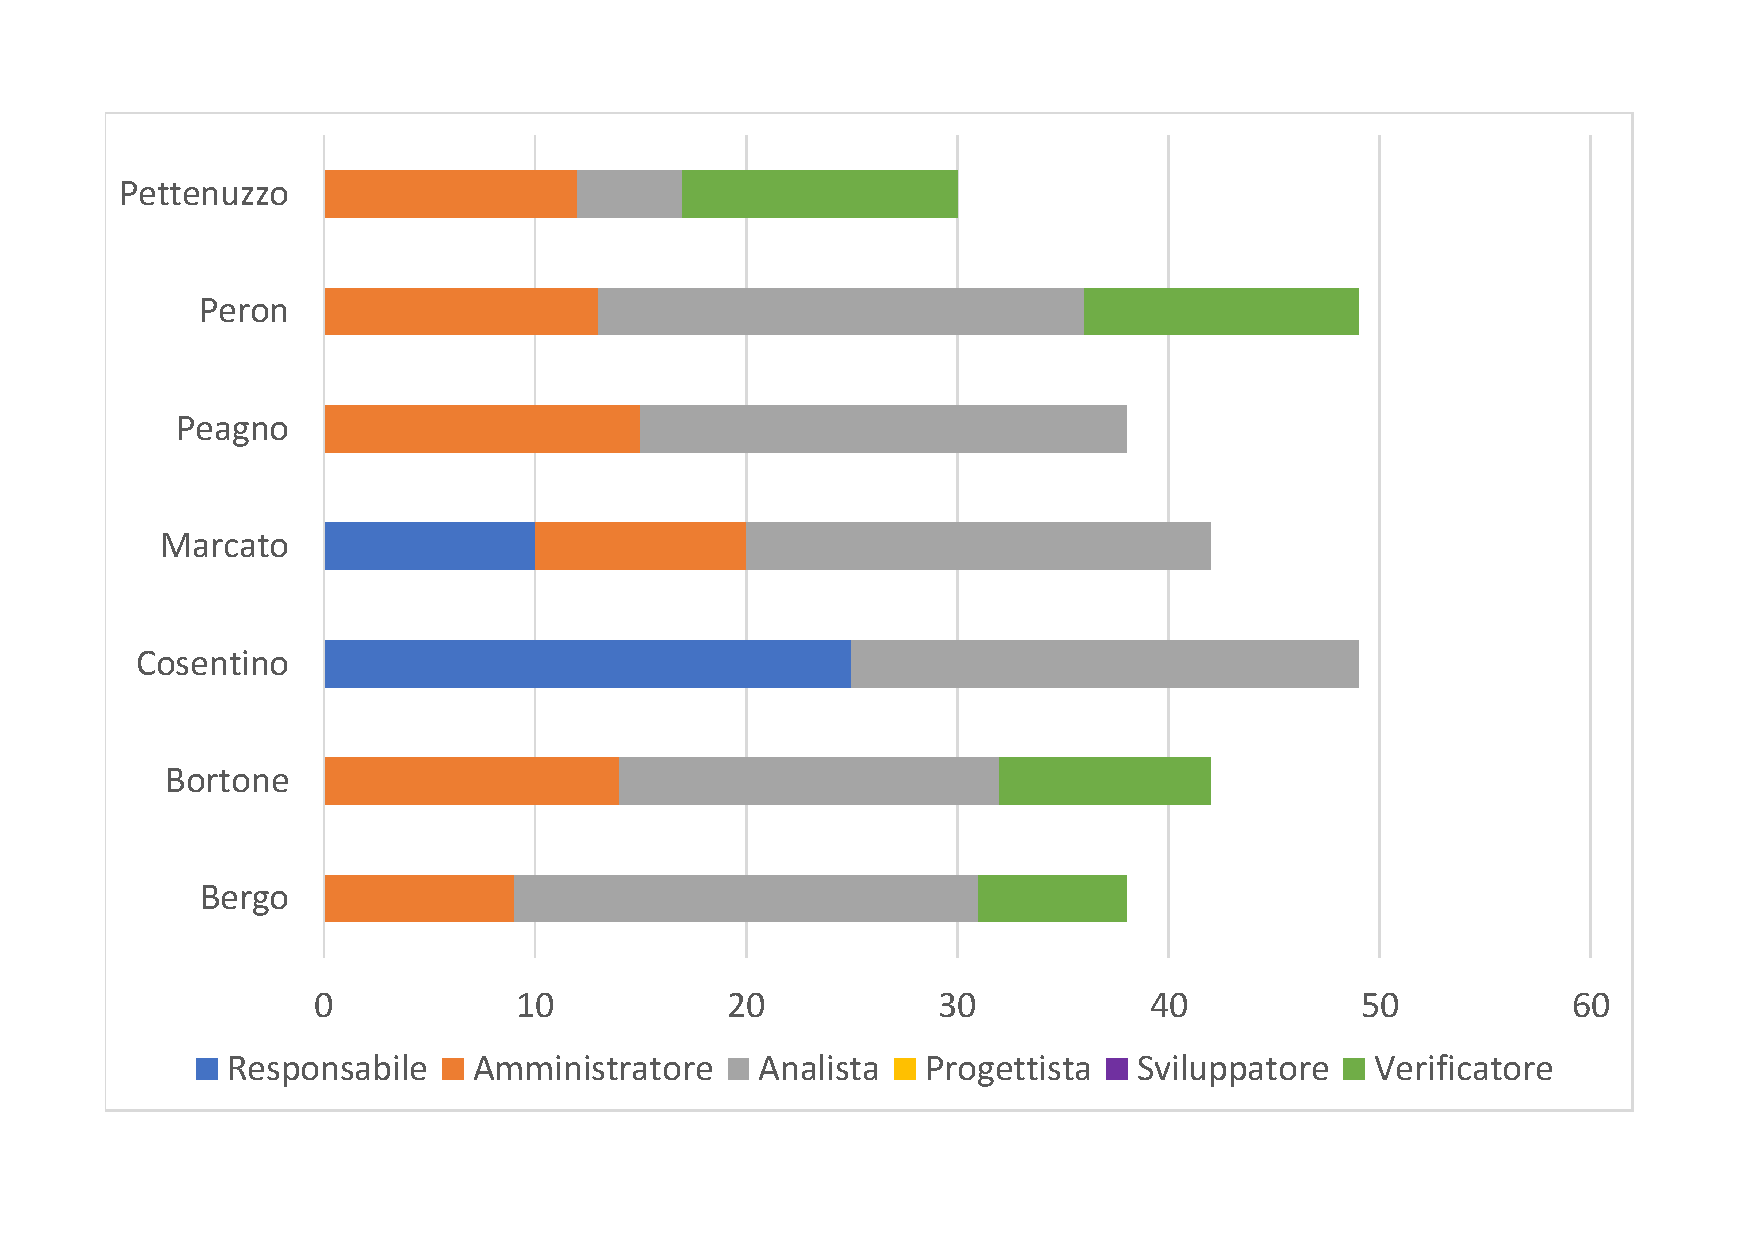
\includegraphics[scale=0.45]{images/consuntivoRR.pdf}
		\caption{Istogramma del consuntivo della fase 1}
	\end{figure}
	
	\subsubsection{Costo}
	Le seguenti tabelle indicano i costi della fase 1. Nell'ultima colonna vengono indicate le differenze tra costi previsti e costi effettivi ($previsto - effettivo$): valori positivi indicano i risparmi e valori negativi indicano le perdite.
	
	\begin{table}[H]
		\centering
		\begin{tabular}{| l | l | l |}
			\rowcolor{LightBlue}
			\textbf{\color{white}Membro}
			& \textbf{\color{white}Costo}
			& \textbf{\color{white}Differenza}\\			
			Bergo 				& 835€ 	& -65€\\
			Bortone 			& 880€ 	& -185€\\
			Cosentino 		& 1350€ 	& -125€\\
			Marcato 			& 1050€ 	& -30€\\
			Peagno 			& 875€ 	& +170€\\
			Peron 				& 1030€ 	& -30€\\
			Pettenuzzo 	& 560€ 	& +290€\\ \hline
			\textbf{Totale} & 6580€ & +25€\\ \hline
		\end{tabular}
		\caption{Costo effettivo di ciascun membro nella fase 1}	
	\end{table}

	\begin{table}[H]
		\centering
		\begin{tabular}{| l | l |l|}
			\rowcolor{LightBlue}
			\textbf{\color{white}Membro}
			& \textbf{\color{white}Costo}
			& \textbf{\color{white}Differenza}\\
			Responsabile 		& 1050€ 	& -150€\\
			Amministratore 	& 1460€ 	& +40€\\
			Analista 				& 3425€ 	& +225€\\
			Progettista 			& 0€ 		& 0€\\
			Programmatore 		& 0€ 		& 0€\\
			Verificatore 		& 645€ 	& -90€\\ \hline
			\textbf{Totale} 	& 6580€ 	& +25€\\ \hline
		\end{tabular}
		\caption{Costo effettivo di ciascun ruolo nella fase 1}
	\end{table}

	\subsubsection{Conclusioni}
		\paragraph{Costi\\}
La cifra prevista per l'investimento era di \textbf{6605€} e vi è stato un risparmio di \textbf{25€}. I costi effettivi ammontano, quindi, a \textbf{6580€}. 
		\paragraph{Scostamenti\\}
Vi sono stati dei leggeri scostamenti rispetto a quanto previsto. Ciò è imputabile a una previsione troppo pessimista delle ore necessarie per ogni attività. Tuttavia, un altro motivo può essere individuato nel mancato rispetto delle assegnazioni delle attività. Ciò è stato causato dalla frenesia da cui si è fatto prendere il gruppo nella parte successiva al periodo natalizio. Infatti, tra il 2018-12-21 e il 2019-01-06 i tempi non sono stati rispettati a causa di problemi di comunicazione tra i membri del gruppo. In seguito, a queste considerazioni è stato aggiunto alla tabella in §2.1 il rischio G03.

\newpage	
\subsection{Fase 2 (2019-01-22 - 2019-03-15)}
	\subsubsection{Ore impiegate}
La seguente tabella indica le ore impiegate durante la fase 2. Tra parentesi viene indicata la differenza tra ore preventivate e ore impiegate ($preventivo - consuntivo$): valori positivi indicano le ore risparmiate e valori negativi indicano le ore in eccesso.

		\begin{table}[H]
			\centering
		\begin{tabular}{| l | c c c c c c | c |}
			\rowcolor{LightBlue}
			& \multicolumn{7}{c}{\textbf{\color{white}Numero di ore}}	\\
	
			\rowcolor{LightBlue}
			\textbf{\color{white}Membro}
			& \textbf{\color{white}RES}
			& \textbf{\color{white}AMM}
			& \textbf{\color{white}AN}
			& \textbf{\color{white}PRO}
			& \textbf{\color{white}DEV}
			& \textbf{\color{white}VER}
			& \textbf{\color{white}Totali}\\
			Bergo     		& -  (0)		& 5  (0) 	& -  (0) 		& 18 (-3) & 10 (0) & 5  (0) 	& 38\\
			Bortone   		& -  (0)		& -  (0) 	& -  (0) 		& 22 (-1) & 9 (0) & -  (0)	& 31\\
			Cosentino 		& -  (0)	 	& -  (0) 	& 7  (-2) 		& 15 (-2) & 5 (0) & 5  (0)	& 32\\
			Marcato   		& -  (0) 		& 10  (0) 	& -  (0) 		& 10 (0) & 7 (0) & 5  (0)	& 32\\
			Peagno    		& -  (0) 		& 8  (0) 	& -  (0) 		& 10 (6) & - (0) & 10  (0)	& 28\\
			Peron     		& 15  (0)		& -  (0) 	& -  (0) 		& 13 (-3) & 10 (0) & -  (0)	& 38\\
			Pettenuzzo 		& 15  (0) 		& -  (0) 	& 8  (2) 		& 7 (-2) & - (0) & -  (0)	& 30\\ \hline
		\end{tabular}
		\caption{Ore di lavoro impiegate per membro/ruolo della fase 1}
	\end{table}
	
	\begin{figure}[H]
		\centering
		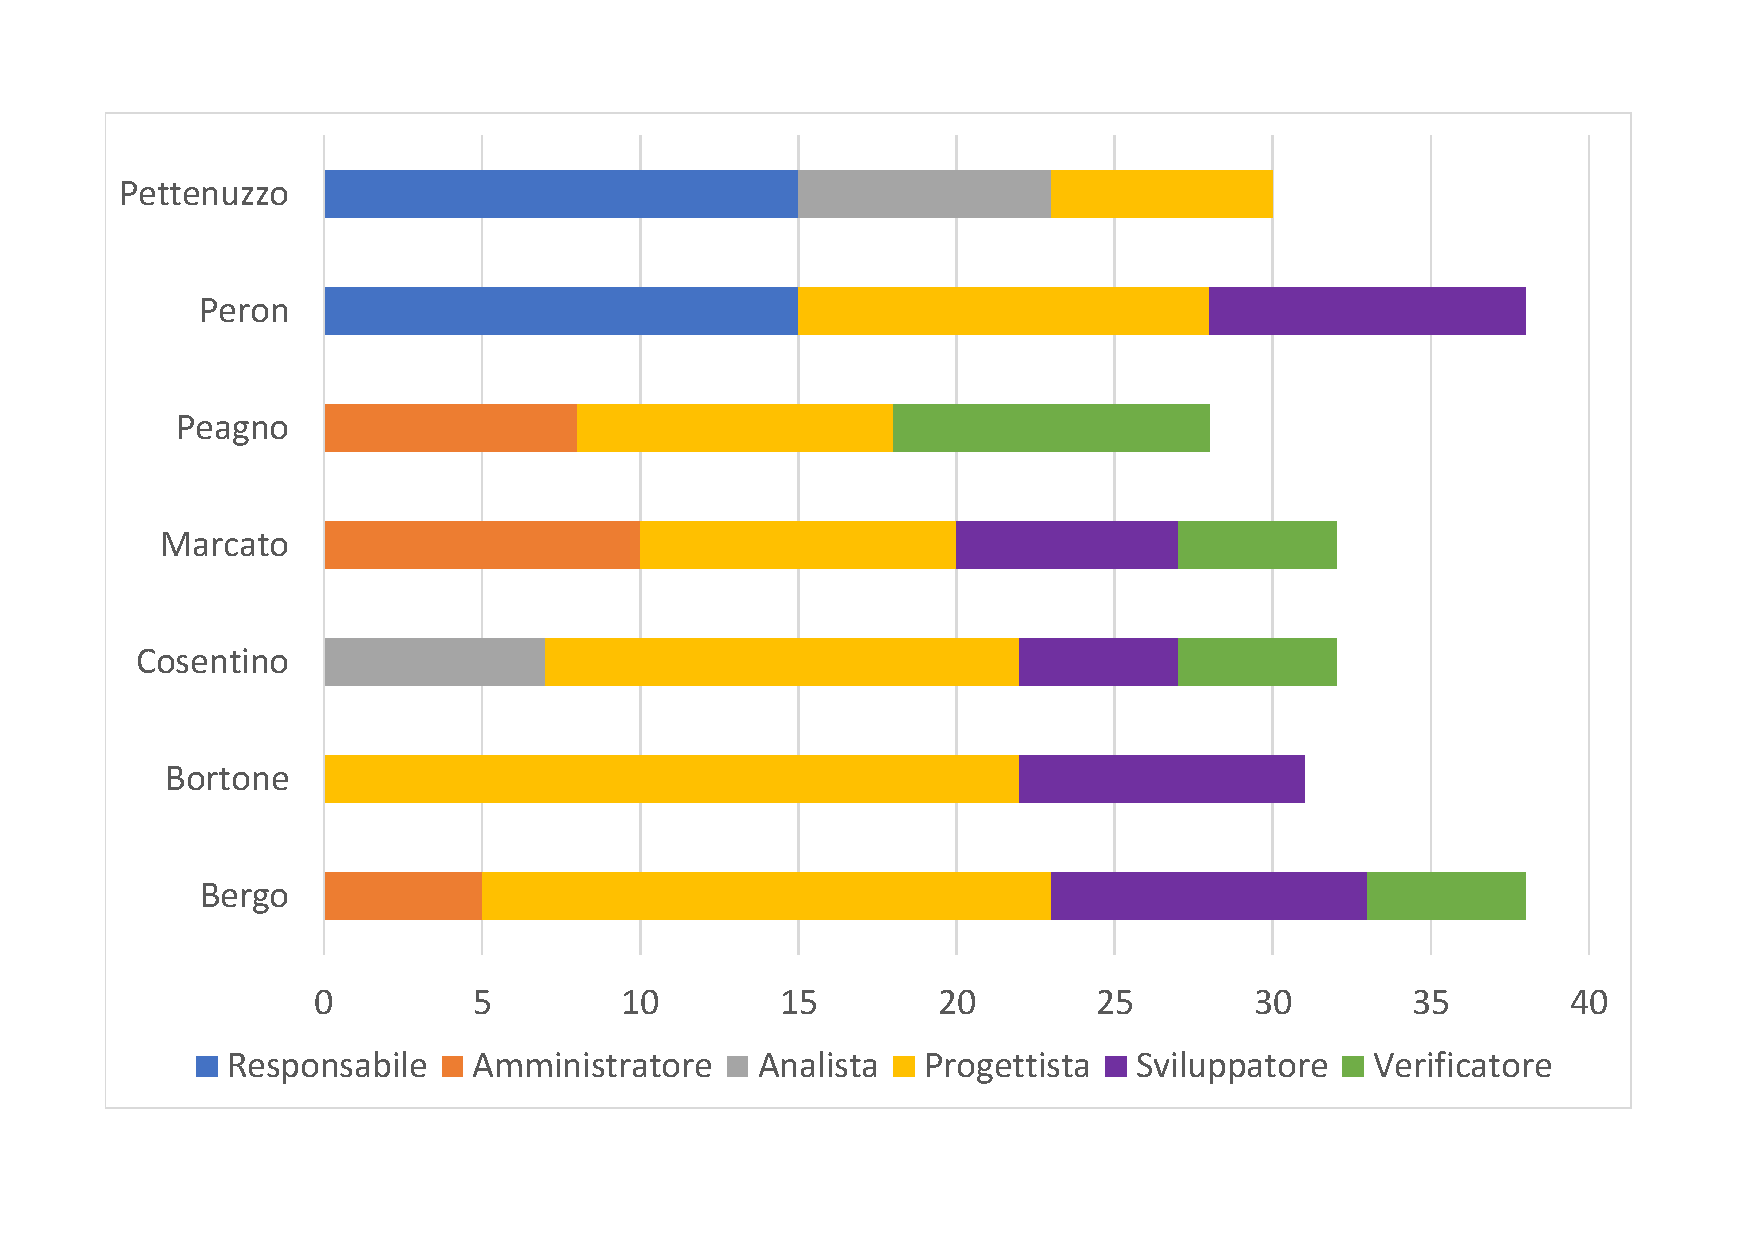
\includegraphics[scale=0.45]{images/consuntivoRP.pdf}
		\caption{Istogramma del consuntivo della fase 2}
	\end{figure}
	
	\subsubsection{Costo}
	Le seguenti tabelle indicano i costi della fase 2. Nell'ultima colonna vengono indicate le differenze tra costi previsti e costi effettivi ($previsto - effettivo$): valori positivi indicano i risparmi e valori negativi indicano le perdite.
		
	\begin{table}[H]
		\centering
		\begin{tabular}{| l | l | l |}
			\rowcolor{LightBlue}
			\textbf{\color{white}Membro}
			& \textbf{\color{white}Costo}
			& \textbf{\color{white}Differenza}\\
			Bergo		& 721€	& 9€\\
			Bortone		& 619€	& 53€\\
			Cosentino	& 655€	& -94€\\
			Marcato		& 600€	& 0€\\
			Peagno		& 530€	& 52€\\
			Peron		& 886€	& -66€\\
			Pettenuzzo	& 804€	& 6€\\ \hline
			\textbf{Totale} & 4815	& -40€\\ \hline
		\end{tabular}
		\caption{Costo effettivo di ciascun membro nella fase 2}	
	\end{table}
	
	\begin{table}[H]
		\centering
		\begin{tabular}{| l | l |l|}
			\rowcolor{LightBlue}
			\textbf{\color{white}Membro}
			& \textbf{\color{white}Costo}
			& \textbf{\color{white}Differenza}\\

			Responsabile	& 900€	& 0€\\
			Amministratore 	& 460€ 	& -80€\\
			Analista 		& 375€ 	& 0€\\
			Progettista 	& 2090€	& -110€\\
			Programmatore 	& 615€	& 150€\\
			Verificatore 	& 375€	& 0€\\ \hline
			\textbf{Totale} & 4815€	& -40€\\ \hline
		\end{tabular}
		\caption{Costo effettivo di ciascun ruolo nella fase 2}
	\end{table}
	
	\subsubsection{Conclusioni}
		\paragraph{Costi\\}
La cifra prevista per l'investimento era di \textbf{4815€}, il costo effettivo si è rivelato con un aumento di \textbf{40€} rispetto alla stima iniziale. Per cui la cifra alla fine della fase 2 corrisponde a \textbf{4770€}.
 		
		\paragraph{Scostamenti\\}
Il gruppo ha riscontrato delle difficoltà nella progettazione del Proof of Concept, la quale ha richiesto più ore rispetto a quanto preventivato. Le difficoltà derivano da una scelta tecnologica che si è rivelata errata per questo motivo sono state prese come alternativa tecnologie già conosciute dai componenti. In questo modo le ore di codifica sono state rispettate in modo soddisfacente senza grandi imprevisti.
\newpage
\subsection{Fase 3 (2019-03-16 - 2019-04-19)}
	\subsubsection{Ore impiegate}
	\subsubsection{Costo}
	\subsubsection{Gestione dei rischi}
	/* Qui si parla dei cambiamenti della tabella analisi dei rischi in base alle fasi precedenti.
	Per esempio la probabilità del rischio legato alla nostra conoscenza è stata abbassata dato che ora ci conosciamo meglio.
	Anche la probabilità legata alla nostra comprensione dei requisiti è stata abbassata dato che siamo in una fase avanzato quindi la nostra comprensione è aumentata
	Poi la comuicazione è migliorata quindi la probabilità del suo rischio è stata abbassata. */
	\subsubsection{Conclusioni}


	\newpage
	\subsection{Preventivo a finire}
La seguente tabella presenta l'attuale preventivo a finire. Se il valore del consuntivo di un determinato periodo non è ancora presente, per il conteggio totale verrà utilizzato il valore del preventivo.

\begin{table}[H]
			\centering
		\begin{tabular}{| l | l | l | l |}
			\rowcolor{LightBlue}
			\textbf{\color{white}Fase}
			& \textbf{\color{white}Preventivo}
			& \textbf{\color{white}Consuntivo}
			& \textbf{\color{white}Variazione}
			\\
			
			Fase 2 			& 4775€ 	& 4815€ & -40€\\
			Fase 3 		& 6353€ 	& - & -\\
			Fase 4			& 3037€ 	& - & -\\
			\textbf{Totale} & 14090€ & 14105€ & -15€\\ \hline
		\end{tabular}
		\caption{Preventivo a finire aggiornato al termine della fase 2}	
\end{table}
La cifra risparmiata durante la fase 1 non è stata reinvestita durante la modifica della pianificazione. La variazione ($preventivo - consuntivo$) quindi è di -15, è necessario un maggiore impegno da parte del gruppo nelle fasi successive per rientrare nel costo preventivato in partenza. 

\newpage